\tikzsetnextfilename{mr_t2_preparation_constants}
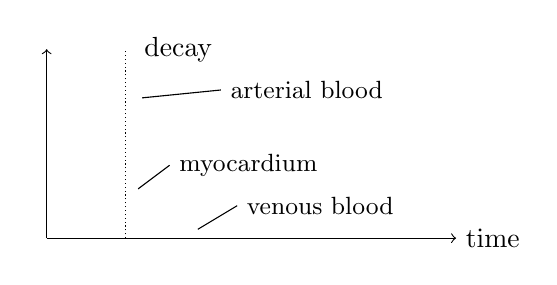
\begin{tikzpicture}[yscale=2]
	\draw[->] (0, 0) -- (0, 1.2) node [left] {\magntrans{}};
	\draw[->] (0, 0) -- (5.2, 0) node [right] {time};
	\draw[densely dotted] (1, 0) -- (1, 1.2) node [right] {\transtime{} decay};
	\draw[domain=0:5,samples=100,very thick] plot[id=mr_t2_arterial] function{exp(-x/10.5)};
	\draw[domain=0:5,samples=100,very thick,densely dotted] plot[id=mr_t2_venous] function{exp(-x*1.5)};
	\draw[domain=0:5,samples=100,very thick,densely dashed] plot[id=mr_t2_myocardium] function{exp(-x)};
	\draw (1.16162, 0.31298) -- +(0.4, 0.15) node [right, font=\small] {myocardium};
	\draw (1.21212, 0.89097) -- +(1, 0.05) node [right, font=\small] {arterial blood};
	\draw (1.91919, 0.05620) -- +(0.5, 0.15) node [right, font=\small] {venous blood};
\end{tikzpicture}